\documentclass[12pt,a4paper]{article}


\usepackage{polyglossia}
\setmainlanguage{french}

\usepackage{amsmath, amssymb}

\usepackage{graphicx}
\usepackage{caption}

\usepackage{siunitx}
\usepackage{myunit}

\usepackage{geometry}
\geometry{top=2cm, bottom=1.5cm, left=2cm, right=1.5cm}
\setlength{\parindent}{0pt}

\usepackage{enumitem}

\usepackage{hyperref}

\usepackage{xcolor}

\usepackage{multicol}
\setlength{\columnseprule}{1pt}
\def\columnseprulecolor{\color{gray}}

\usepackage{tcolorbox}


\usepackage{import}
\usepackage{xifthen}
\usepackage{pdfpages}
\usepackage{transparent}
\usepackage{float}

\newcommand{\incfig}[1]{%
	\def\svgwidth{\columnwidth}
	\import{./figures/}{#1.pdf_tex}
}


\newcommand{\RomanNum}[1] %pour les chiffre romain
{\MakeUppercase{\romannumeral #1}}





\usepackage{stanli}
\usetikzlibrary{patterns}

\usepackage{ae,aecompl}
\usepackage{listings}


\usepackage{tikz-dimline}


























\title{Ouvrages spéciaux : TD 2 passerelle en BA}
\author{}
\date{\today}

\begin{document}
	\counterwithin{section}{part} % pour que \section{} recommence de 1 aprés \part{}
	
	\maketitle
	
	\tableofcontents
	
	\newpage
	
	
	\part{Exo 2}
	
	
	
	
	
	
	
	
	
	\section{Rappel pour un trapèze}
	
	\begin{multicols}{2}
		
		
		\[ S = \dfrac{B + b}{2} \cdot h \]
		
		\[ V_{1} = \dfrac{h \cdot (2B + b)}{3 \cdot (B + b)} \]
		
		\[ V_{2} = \dfrac{h \cdot (B + 2b)}{3 \cdot (B + b)} \]
		
		
		\columnbreak
		
		\begin{figure}[H]
			\centering
			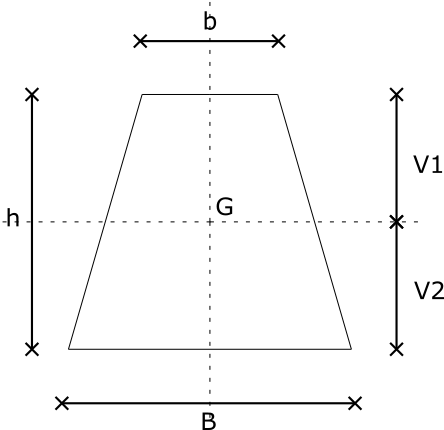
\includegraphics[width=0.7\linewidth]{figures/rappel-trapeze}
		\end{figure}
		
		
	\end{multicols}
	
	
	
	
	
	
	
	
	
	
	
	
	
	
	
	
	
	
	\section{Vérification au renversement}
	
	Vérifions que l'ouvrage ne risque pas de basculer autour du point A lorsqu'il n'est chargé que d'un seul coté.
	
	\vspace{\baselineskip}
	
	\begin{tikzpicture}[scale=0.3]
		
		
		\draw (0,0)
		-- (3,0) coordinate (A)
		-- ++(0,4)
		-- ++(5,3)
		-- ++(0,3) coordinate (B);
		
		\draw (0,0)
		-- (0,4)
		-- ++(-5,3)
		-- ++(0,3)
		-- (B);
		
		
		\fill (A) circle (10pt) node[right] {\Huge \textcolor{red}{A}};
		
		
	\end{tikzpicture}
	
	
	
	
	
	
	
	\subsubsection{Calcul du poids propre au 1ml}
	
	\begin{itemize}
		\item Garde du corps (des deux coté) : $ = 40 ~\unit{kg}$
		\item Murettes : $ = 2 \cdot (0,1 \cdot 0,1) \cdot 2500 = 50 ~\unit{kg}$
		\item Console : $ = 2 \cdot \left( \dfrac{0,12 + 0,08}{2} \cdot 0,8 \right) \cdot 2500 = 400 ~\unit{kg}$
		\item Poutre : $ = (0,4 \cdot 0,1) \cdot 2500 = 1000 ~\unit{kg}$
		
		\item Revetement : $ = 1,8 \cdot 100 = 180 ~\unit{kg}$
	\end{itemize}
	
	\[ P = 1670 ~\unit{kg} \text{ pour 1ml} \]
	
	
	\subsubsection{Surcharge}
	
	\[ S = 500 \cdot 1 \cdot 0,7 = 350 ~\unit{kg} \]
	
	
	
	
	\begin{figure}[H]
		\centering
		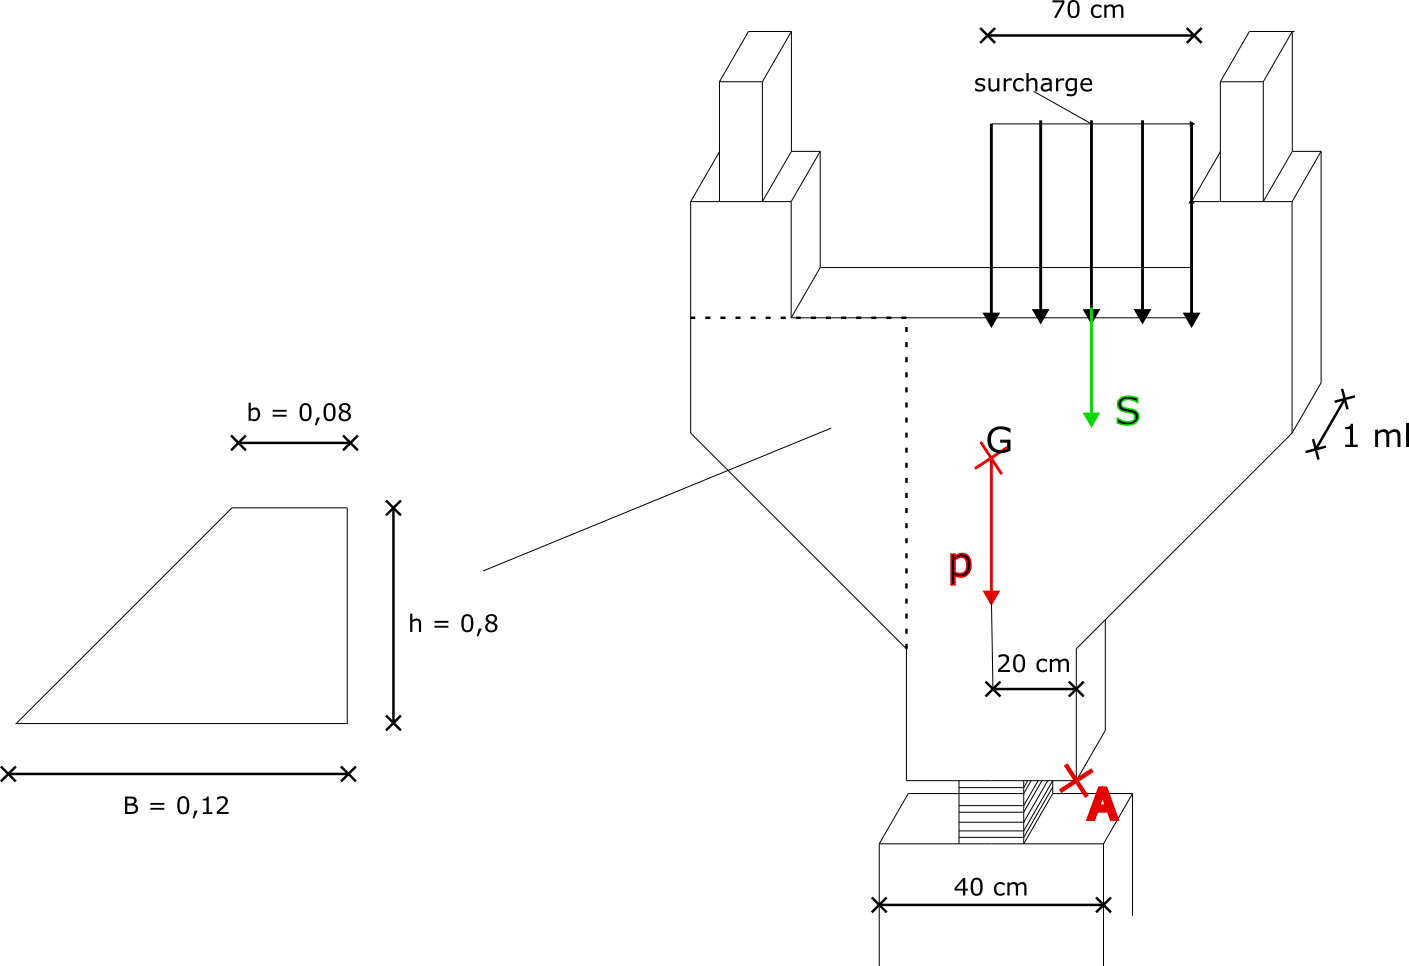
\includegraphics[width=1\linewidth]{figures/poutre-te}
	\end{figure}
	
	
	
	\subsubsection{Moments stabilisant}
	
	\[ M_{s} = M_{/a}\circlearrowleft = P \cdot 0,2 = 1670 \cdot 0,2 = 334 \]
	
	\[ \fbox{$M_{s} = 334 ~\unit{kgm}$} \]
	
	
	\subsubsection{Moments reversant}
	
	\[ M_{r} = M_{/a}\circlearrowright = S \cdot 0,35 = 350 \cdot 0,35 = 122,5 \]
	
	\[ M_{r} = 122,5 ~\unit{kg} \]
	
	
	\subsubsection{Sécurité au renversement}
	
	\[ \begin{aligned}
		M_{s} &> 1,5 \cdot M_{r} \\
		334 &> 1,5 \cdot 122,5 = 183,75\\
	\end{aligned} \]
	 
	
	{\centering Condition vérifier le système est stable. \par}
	
	
	
	
	
	
	\section{Calcul des armatures des éléments de la passerelle en BA a \textbf{l'ELU}}
	
	
	\subsection{Armature de la dalle en console}
	
	\subsubsection{Évaluation des moments reversant a une console}
	
	
	\begin{figure}[H]
		\centering
		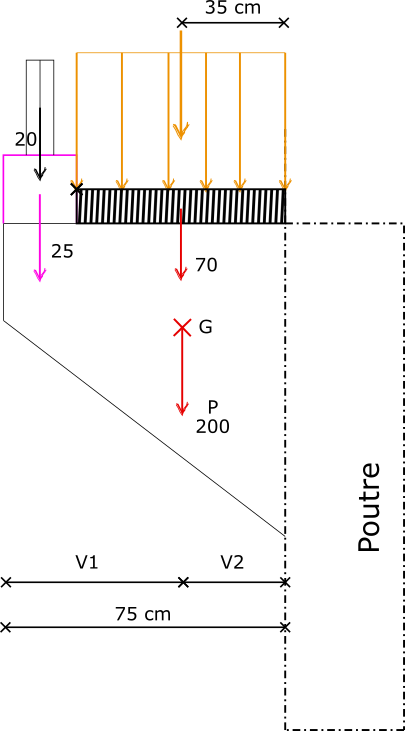
\includegraphics[width=0.45\linewidth]{figures/poutre-te2}
		\caption{}
		\label{fig:poutre-te2}
	\end{figure}
	
	
	
	\begin{itemize}
		\item Garde corp (un seul coté) $ = 1,35 \cdot \dfrac{40}{2} \cdot 0,75 = 20,25 ~\unit{kgm}$
		
		\item Murrette $ = 1,35 \cdot \dfrac{400}{2} \cdot V_{2} = 1,35 \cdot 200 \cdot 0,375 = 101,25 ~\unit{kgm}$
		\subitem $V_{2} = \dfrac{h \cdot (B + 2b)}{3 \cdot (B + b)} = \dfrac{0,8 \cdot (2 \cdot 0,08 + 0,12)}{3 \cdot (0,12 + 0,08)} = 0,375 ~\unit{m}$
		
		\item Revêtement $ = 1,35 \cdot 100 \cdot 0,7 \cdot 0,35 = 33,075 ~\unit{kgm}$
		
		\item Surcharge $ = 1,5 \cdot 500 \cdot 0,7 \cdot 0,35 = 183,75 ~\unit{kgm}$
		
		 
	\end{itemize}
	
	On somme et on a :
	
	\[ \fbox{$M_{ELU} = 363,7563 ~\unit{kgm}$} \]
	
	
	
	
	\subsubsection{Ferraillage (armature principale)}
	
	Fissuration préjudiciable $\rightarrow c = 3 ~\unit{cm}$
	
	La hauteur utile $\rightarrow d = h - c = 12 - 3 = 9 ~\unit{cm}$
	
	\[ \mu = \dfrac{M_{\max}}{b \cdot d^{2 \cdot f_{bu}}} = \dfrac{363,6375 \cdot 10 \cdot 10^{2}}{100 \cdot 9^{2} \cdot 14,2 \cdot 10^{2}} \]
	
	\[ \mu = 0,0316 \]
	
	\[ \mu = 0,0316 < \mu_{l} = 0,392 \rightarrow SSA \]
	
	\vspace{\baselineskip}
	
	Par interpolation : $\beta = \beta_{1} + (\beta_{2} - \beta_{1}) \cdot \dfrac{(\mu - \mu_{1})}{(\mu_{2} - \mu_{1})}$
	
	Pour $\mu = 0,0316 \rightarrow \beta = 0,9839$
	
	\[ A_{st} = \dfrac{M_{ELU}}{\beta \cdot d \cdot \sigma_{st}} = \dfrac{363,7563 \cdot 10^{3}}{0,9839 \cdot 9 \cdot \dfrac{400}{1,15} \cdot 10^{2}} = 1,18 ~\unit{cm^{2}} \]
	
	Nous prendrons 5HA8 $ = 2,51 ~\unit{cm^{2}}$ avec un espacement de 20cm.
	
	
	
	\paragraph{Condition non fragilité}
	
	\[ A_{st} > A_{\min} = \dfrac{0,23 \cdot b \cdot d \cdot f_{t28}}{f_{e}} = \dfrac{0,23 \cdot 100 \cdot 9 \cdot 2,1}{400} = 1,086 ~\unit{cm^{2}} \]
	
	\[ A_{st_{adoptée}} = 2,51 ~\unit{cm^{2}} > A_{\min}  = 1,086 ~\unit{cm^{2}} \]
	
	{\centering Condition vérifiée \par}
	
	\vspace{\baselineskip}
	
	
	
	Armature de répartition : 
	
	\[ A_{r} = \dfrac{A_{st}}{4} = \dfrac{2,51}{4} = 0,6295 ~\unit{cm^{2}} \]
	
	Nous prendrons 4HA8 $ = 2,01 ~\unit{cm^{2}}$ avec un espacement 25cm.
	
	
	\subsubsection{Effort tranchant max agissant sur l'appuie}
	
	\[ V_{\max} = 70 + 350 + 20 + 25 + 200 = 665 ~\unit{kg} \]
	
	\begin{center}
		
	
	\begin{tikzpicture}
		
		\draw (0,0)
		-- (5,0)
		-- (5,0.5) -- (5,-0.5) -- ++(0.1,0.1);
		\draw (5,0) coordinate (a);
		\draw (5,0.1) coordinate (b);
		\draw (5,0.2) coordinate (c);
		\draw (5,-0.1) coordinate (d);
		\draw (5,-0.2) coordinate (e);
		
		\draw (a) -- ++(0.1,0.1);
		\draw (b) -- ++(0.1,0.1);
		\draw (c) -- ++(0.1,0.1);
		\draw (d) -- ++(0.1,0.1);
		\draw (e) -- ++(0.1,0.1);
		
		\draw[->,thick] (0,0) -- (0,-1) coordinate(A);
		\draw[<-,thick] (0,0) -- (0,1) coordinate(B);
		\draw[->,thick] (2,0) -- ++(0,-1) coordinate(C);
		\draw[<-,thick] (3,0) node[right] {350 ~\unit{kg}} -- (3,1) coordinate(D);
		\draw[<-,thick] (D) -- ++(0,1) coordinate(E);
		
		\fill (A) node[right] {25 ~\unit{kg}};
		\fill (B) node[right] {20 ~\unit{kg}};
		\fill (C) node[right] {200 ~\unit{kg}};
		\fill (E) node[right] {25 ~\unit{kg}};
		
	\end{tikzpicture}
	
	
	
	\end{center}
	
	
	\subsubsection{Calcul des contrainte tangentielle}
	
	\[ \tau_{u} = \dfrac{V_{\max}}{b_{0} \cdot d} = \dfrac{665 \cdot 10}{1000 \cdot 90} = 0,0738 ~\unit{MPa} \]
	
	Fissuration préjudiciable : 
	
	\[ \overline{\tau}_{u} = \min \left.\begin{cases}
		0,05 \cdot f_{c28} = 0,05 \cdot 30 = 1,5 ~\unit{MPa} \\
		5 ~\unit{MPa}
	\end{cases}\right\} \rightarrow \overline{\tau}_{u} = 1,5 ~\unit{MPa} \]
	
	\[ \tau_{u} = 0,073 ~\unit{MPa} < \overline{\tau}_{u} = 1,5 ~\unit{MPa} \]
	
	{\centering Condition vérifié \par}
	
	
	\vspace{\baselineskip}
	
	\[ V_{\max} + \dfrac{M_{ELU}}{0,9d} = 665 + \dfrac{ - 363,7563}{0,9 \cdot 0,09} =  - 3824,35 < 0 \]
	
	{\centering Condition vérifiée \par}
	
	
	
	
	
	
	
	
	
	
	\subsection{Armature de la poutre}
	
	\subsubsection{Évaluation de la charge}
	
	\begin{center}
		
	
		\begin{tikzpicture}
			
			
			\draw[pattern=north west lines] (0,0) rectangle (3,.5) node[midway, red] 	{revêtement};
			\draw (0,0) rectangle (3,-4) node[midway]{poutre};
			\foreach \xlin in {0,0.5,...,3}
			\draw[->, ultra thick] (\xlin,1) -- (\xlin,0);
			\draw (0,1) -- (3,1) node[above, midway]{Revêtement = 100};
			\foreach \xlin in {0,0.5,...,3}
			\draw[->, ultra thick] (\xlin,3) -- (\xlin,1.5);
			\draw (0,3)--(3,3) node[above, midway]{Suracharge = 500};
			\draw[->, ultra thick] (-0.5,-3) -- (-0.5,-1);
			\draw[<-, ultra thick] (-1,-3) -- (-1,-1) node[midway, left]{$R_{1} = 	V_{\max}$};
			\draw[->, ultra thick] (3.5,-3) -- (3.5,-1);
			\draw[<-, ultra thick] (4,-3) -- (4,-1) node[midway, right]{$R_{1} = 	V_{\max}$};
			\draw[|-|, thick] (0,-5) -- (3,-5) node[midway, above]{$40 ~\unit{cm}$};
			
		\end{tikzpicture}
	
	
	\end{center}

	\vspace{\baselineskip}
	
	\begin{itemize}
		\item Réactions des console $ = 2 \cdot V_{\max} = 2 \cdot 665 = 1330 ~\unit{kg}$
		\item P.P de la poutre $ = 1 \cdot 0,4 \cdot 2500 = 1000 ~\unit{kg}$
		\item Revêtement de la poutre $100 \cdot 0,4 = 40 ~\unit{kg}$
		\item Surcharge sur la poutre $ = 500 \cdot 0,4 = 200 ~\unit{kg}$
	\end{itemize}
	
	\[ P_{poutre}^{ELU} = 1,35 \cdot (1330 + 1000 + 40) + 1,5 \cdot 200 \]
	
	\[ \fbox{$P_{_{poutre}ELU} = 3499,5 ~\unit{kg}$} \]

	
	
	
	\subsubsection{Calcul section té (position l'axe neutre)}
	
	\[ \text{Moment max : } M_{\max} = \dfrac{Pl^{2}}{8} = \dfrac{3499,5 \cdot 10^{2}}{8} = 43743,75 ~\unit{kgm} \]
	
	\vspace{\baselineskip}
	
	\begin{minipage}{0.7\textwidth}
		\paragraph{Le moment équilibrée par la table de compression}
		
		\[ M_{tab} = f_{bu} \cdot b \cdot h_{0} \cdot (d - \dfrac{h_{0}}{2}) = 14,2 \cdot 10^{5} \cdot 2 \cdot 0,1 \cdot (0,96 - \dfrac{0,1}{2}) \]
		
		\[ M_{tab} = 258440 ~\unit{kgm} \]
	\end{minipage}
	\begin{minipage}{0.3\textwidth}
		
		\begin{tikzpicture}[scale=0.8]
			
			\draw (0,0) -- (4,0) -- ++(0,-1) -- ++(-1.2,-1) -- ++(0,-2.3) coordinate(a);
			\draw (0,0) -- (0,-1) -- ++(1.2,-1) -- ++(0,-2.3) -- (a);
			
			\draw[|-|] (-.5,0) -- (-.5,-1) node[midway,left]{8};
			\draw[|-|] (0,.5) -- (4,.5) node[midway,above]{200};
			\draw[|-|] (4.5,0) -- (4.5,-3.8) coordinate (b) node[midway,right]{96};
			\draw[|-|] (b) -- ++(0,-0.5) node[midway,right]{4};
			\draw[|-|] (5.5,0) -- (5.5,-4.3) node[midway,right]{100};
		\end{tikzpicture}
		
	\end{minipage}


	\[ M_{ELU} = 43743,75 \quad<\quad M_{tab} = 258440 \]
	
	L'axe neutre se trouve dans la table de compression, le calcul se fera on considérant une section rectangulaire $b \times h = 200 \times 100$

	\subsubsection{Calcul du ferraillage}

	\[ \mu = \dfrac{M_{ELU}}{b \cdot d^{2} \cdot f_{bu}} = \dfrac{33743,75 \cdot 10 \cdot 10^{2}}{200 \cdot 96^{2} \cdot 14,2 \cdot 10^{2}} = 0,0167 \]
	
	\[ \mu = 0,0167 < \mu_{l} = 0,392 \rightarrow SSA \]
	
	{\centering Par interpolation on aura : \par}
	
	\[ \beta = \beta_{1} + (\beta_{2} - \beta_{1})\dfrac{(\mu - \mu_{1})}{(\mu_{2} - \mu_{1})} \]

	\[ \beta = 0,9915 \]
	
	\vspace{\baselineskip}
	
	\[ A_{st} = \dfrac{M_{\max}}{\beta \cdot d \cdot \sigma_{st}} = \dfrac{43743,75 \cdot 10^{3}}{0,9915 \cdot 96 \cdot \dfrac{400}{1.15} \cdot 10^{2}} \]
	
	\[ A_{st} = 13,206 ~\unit{cm^{2}} \]
	
	Nous prendrons : $A_{st} = 5HA20 = 15,7 ~\unit{cm^{2}}$
	
	
	\subsubsection{Condition non fragilité}
	
	\subsubsection{L'effort tranchant au appuie}
	
	\[ V_{\max} = \dfrac{P_{ELU} \cdot l}{2} = \dfrac{3499,5 \cdot 10}{2} = 17497,5 ~\unit{kg} \]
	
	
	\paragraph{Contrainte tangentielle}
	
	\[ \tau_{u} = \dfrac{V_{\max}}{b_{0}d} = \dfrac{17497,5 \cdot 10}{400 \cdot 960} = 0,455 ~\unit{MPa} \]
	
	{\centering Fissuration préjudiciable\par}
	\[ \downarrow \]
	
	\[ \overline{\tau}_{u} = \min\left.\begin{cases}
		0,2\dfrac{f_{c28}}{\gamma_{b}} \\
		5 ~\unit{MPa}
	\end{cases}\right\} = 3,33 ~\unit{MPa} \]
	
	\[ \tau_{u} < \overline{\tau}_{u} \]
	{\centering condition vérifiée}
	
	
	
	\subsubsection{Vérification pour poutre a nervure rectangulaire}
	
	Dans le cas de la poutre a nervure rectangulaire, on doit vérifier que :
	
	\[ V_{\max} < 0,237 \cdot b \cdot a \cdot f_{c28} \]
	
	Poutre sur appareil d'appuis : $a = 4 + 20 + 4 = 28 ~\unit{cm}$
	
	\begin{center}
		\begin{tikzpicture}
			
			\draw (0.8,1) coordinate(a) -- (0,1) -- (0,0) -- (3,0) -- (3,1) -- (2.2,1);
			
			\draw[pattern=horizontal lines] (a) rectangle (2.2,2);
			
			\draw[|-|] (0,2.5) -- (0.8,2.5) node[midway,above]{4} coordinate(b);
			\draw[|-|] (b) -- (2.2,2.5) node[midway,above]{20} coordinate(c);
			\draw[|-|] (c) -- (3,2.5) node[midway,above]{4};
			
		\end{tikzpicture}
	\end{center}
	
	
	\[ V_{\max} = 174975 ~\unit{N} < 0,237 \cdot 400 \cdot 280 \cdot 25 = 592500 ~\unit{N} \]
	
	{\centering Condition vérifier\par}
	
	
	\subsubsection{Armature transversale}
	
	Les armatures transversal seront constituée par un cadre et deux epingle HA6 $\rightarrow A_{t} = 1,13 ~\unit{cm^{2}}$
	
	Les espacement des armatures doit vérifier les conditions suivante : 
	
	\[ S_{t} \leq \min \left.\begin{cases}
		0,9 \cdot d \\
		40 ~\unit{cm}
	\end{cases}\right\}  = 40 ~\unit{cm} \]

	\[ S_{t} \leq \dfrac{A_{t} \cdot f_{e}}{0,4 \cdot b} = \dfrac{1,13 \cdot 400}{0,4 \cdot 40} = 28,25 ~\unit{cm} \]
	
	
	
	
	
	
	
	
	
	\section{Calcul des éléments de la passerelle en BA a \textbf{ELS}}
	
	
	\[ \overline{\sigma}_{bc} = 0,6 \cdot f_{c28} = 15\mpa \]
	
	
	Fissuration préjudiciable $\rightarrow \overline{\sigma}_{st} = \min \left. \begin{cases}
	\dfrac{2}{3}f_{e} \\
	110\sqrt{n \cdot f_{tj}} \text{ avec $n = 1.6$ pour les barres HA. }
	\end{cases}\right\}$ 
	
	\[ \overline{\sigma}_{st} = \min \{ 266,66 \quad;\quad 201,688  \} = 201,633\mpa \]
	
	
	
	\subsection{Armature de la dalle en console}
	
	\subsubsection{Évaluation du moments a l'ELS}
	
	Évaluation des moments renversant à une console : 
	
	\begin{itemize}
		\item Garde corps (d'un seul coté) $ = 20 \cdot 0,75 = 15\kgxm$
		\item Murette $ = 25 \cdot 0,75 = 18,75\kgxm$
		\item Console $200 \cdot 0,375 = 75\kgxm$
		\item Revêtement $70 \cdot 0,35 = 24,5\kgxm$
		\item Surcharge $350 \cdot 0,35 = 122,5\kgxm$
	\end{itemize}
	
	\[ M_{ELS} = 255,75\kgxm \]
	
	
	
	
	\begin{tikzpicture}
		
		
		\point{a}{0}{0};
		\point{b}{3}{0};
		\point{c}{3}{3};
		\point{d}{1}{3};
		\point{g}{1.9}{1.2};
		
		\beam{2}{a}{b};
		\beam{2}{b}{c};
		\beam{2}{c}{d};
		\beam{2}{d}{a};
		
		\dimensioning{1}{a}{b}{-.8}[B];
		\dimensioning{1}{c}{d}{-1.7}[b];
		
		\dimensioning{2}{a}{g}{-.8}[$V_{1}$];
		\dimensioning{2}{g}{d}{-.8}[$V_{2}$];
		
		\notation{2}{g}{G};
		
	\end{tikzpicture}
	
	
	
	\begin{tikzpicture}
		
		
		\point{a}{0}{0};
		\point{b}{1}{0};
		\point{cc}{1}{-1};
		\point{c}{6}{-1};
		\point{d}{6}{-6};
		\point{e}{0}{-3};
		
		
		\point{A}{.5}{.5};
		\point{B}{.5}{-1.5};
		
		\point{C}{3.5}{-.5};
		\point{D}{3.5}{-2};
		
		\point{G}{4.5}{-3};
		
		
		\beam{2}{a}{b};
		\beam{2}{b}{cc};
		\beam{2}{cc}{c};
		\beam{2}{c}{d};
		\beam{2}{d}{e};
		\beam{2}{e}{a};
		
		
		\load{1}{A}[90];
		\notation{1}{A}{20 garde corps};
		
		\load{1}{B}[90];
		\notation{1}{B}{25 murette};
		
		\load{1}{C}[90];
		\notation{1}{C}{350 surcharge};
		
		\load{1}{D}[90];
		\notation{1}{D}{70 Revêtement};
		
		\load{1}{G}[90];
		\notation{1}{G}{G 200};
		
		
		\dimensioning{1}{A}{c}{-9}[$75\cml$];
		\dimensioning{1}{C}{c}{-8}[$35\cml$];
		\dimensioning{1}{G}{c}{-7}[$V_{2} = 37,5\cml$];
		
		
		\draw[pattern,pattern=north west lines] (1,-1) rectangle (6,-.5) node[midway]{Revêtement};
		
		\draw (.2,0) rectangle (.7,1);
		
	\end{tikzpicture}
	
	
	
	
	
	
	
	
	
	
	
	
	
	
	
\end{document}